When trained, the model for 300 epochs with a batch size of 50, it showed an accuaracy of:
\begin{itemize}
      \item Training Set:
        \begin{itemize}
            \item First epochs: 32,8\%
            \item Last epoch: 98,6\%
        \end{itemize}
      \item Test Set:
        \begin{itemize}
            \item First epochs: 38,8\%
            \item Last epoch: 46,9\%
        \end{itemize}
\end{itemize}
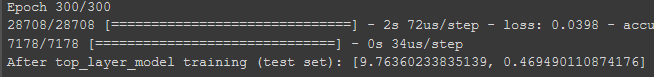
\includegraphics[scale=0.9]{images/modelOne/evaluationOne.png}
Test/Validation Set above suggest that mode is over-fitting.\\
\\
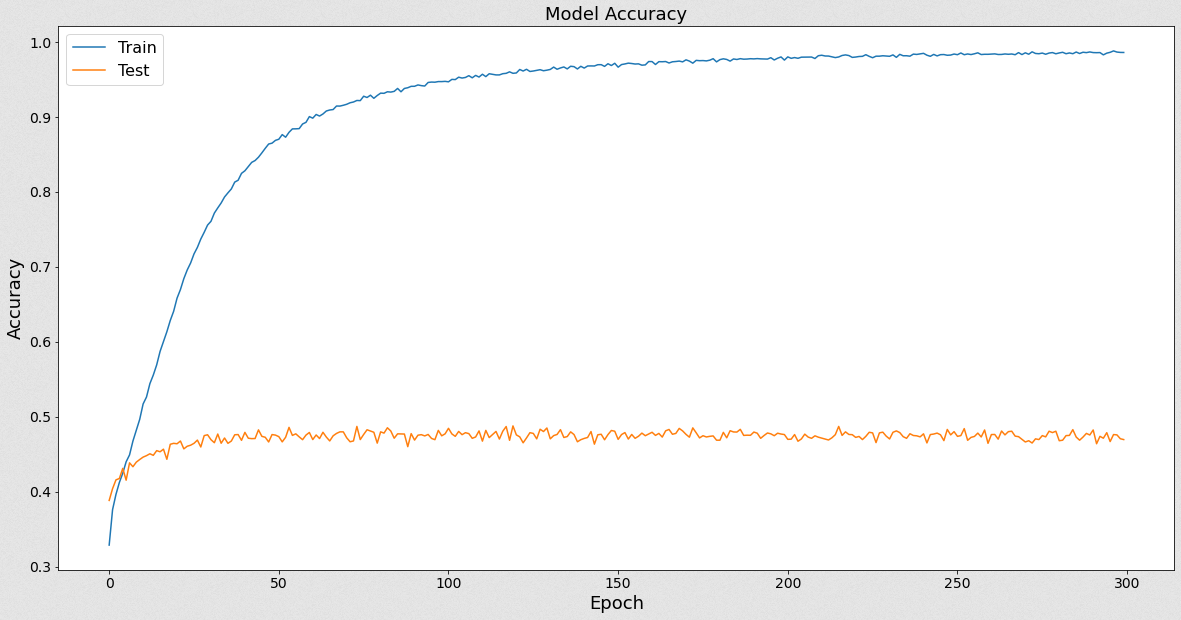
\includegraphics[scale=0.5]{images/modelOne/accOne.png}
Accuracy on the train set is steadily increasing, but on the test set it increases only in the first thirty-forty epochs. Difference in accuracy is likely caused by over-fitting. In real life accuracy will probably be even lower, due to problems like different face position, or bad light.  By doing some preprocessing on new images to more closely match the images fed in during training/testing - this should increase accuracy.\\
\\
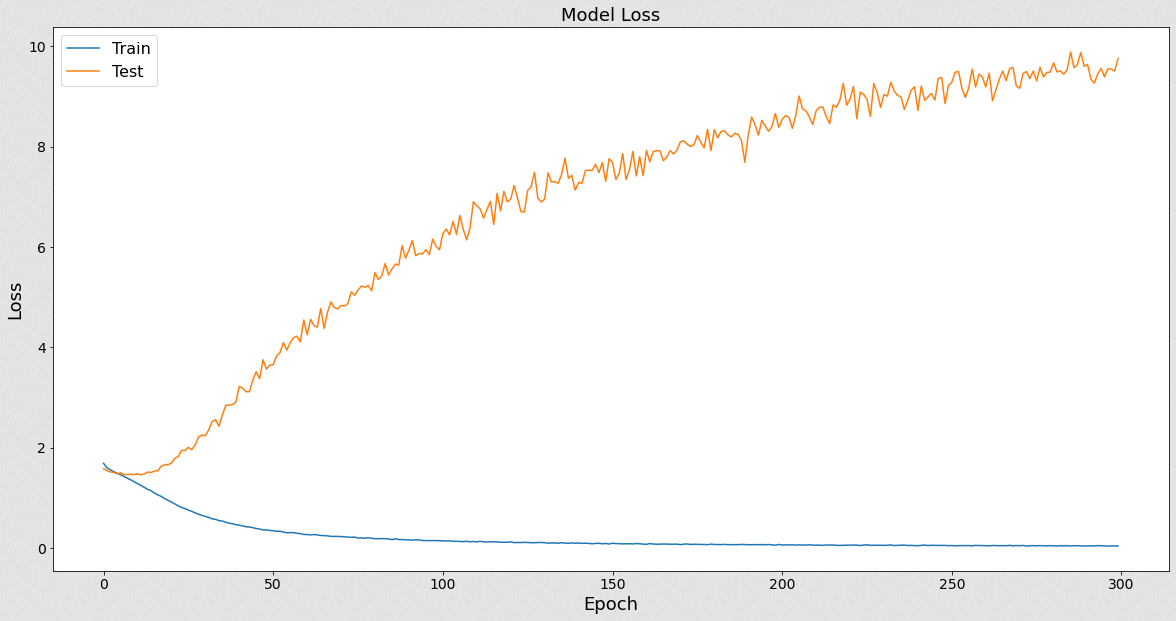
\includegraphics[scale=0.5]{images/modelOne/lossOne.png}
Validation loss is much higher than training loss, which proves our theory about over-fitting\\
\\
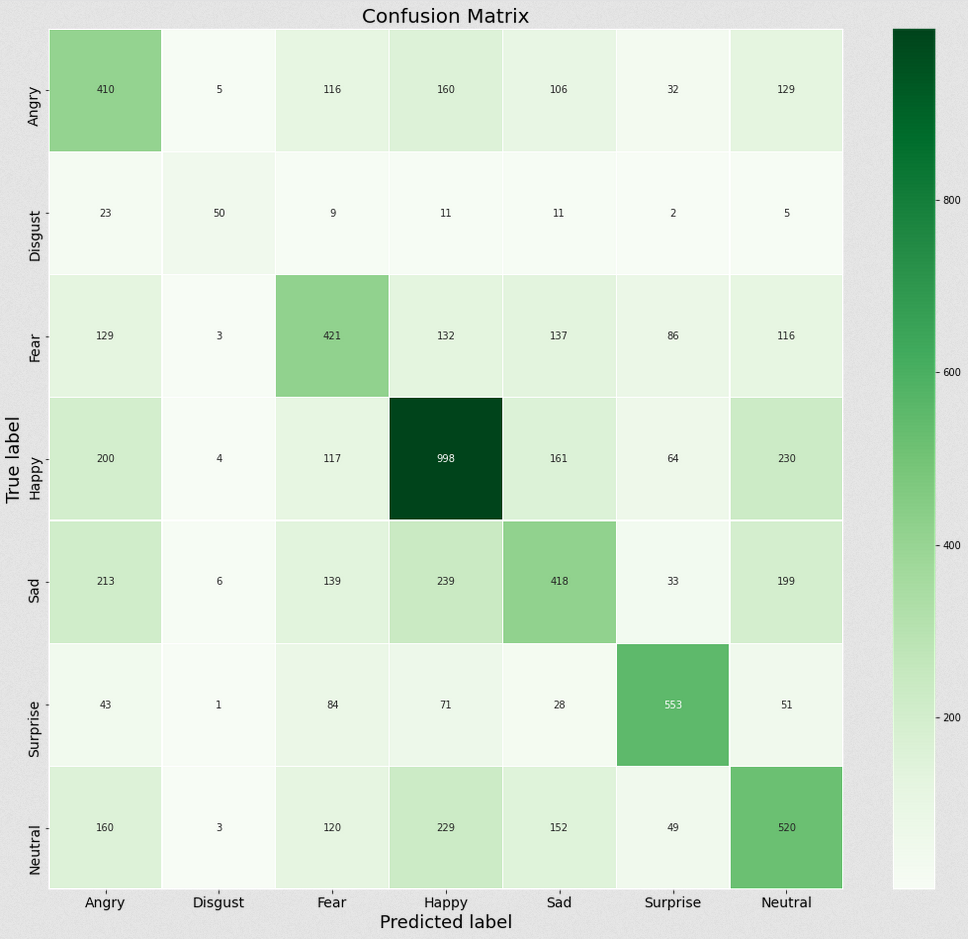
\includegraphics[scale=0.60]{images/modelOne/matrixOne.png}\\
Confusion matrix shows us mistakes that model made.\\
\\
Here are some examples:
\begin{itemize}
    \item Correctly predicted images\\
            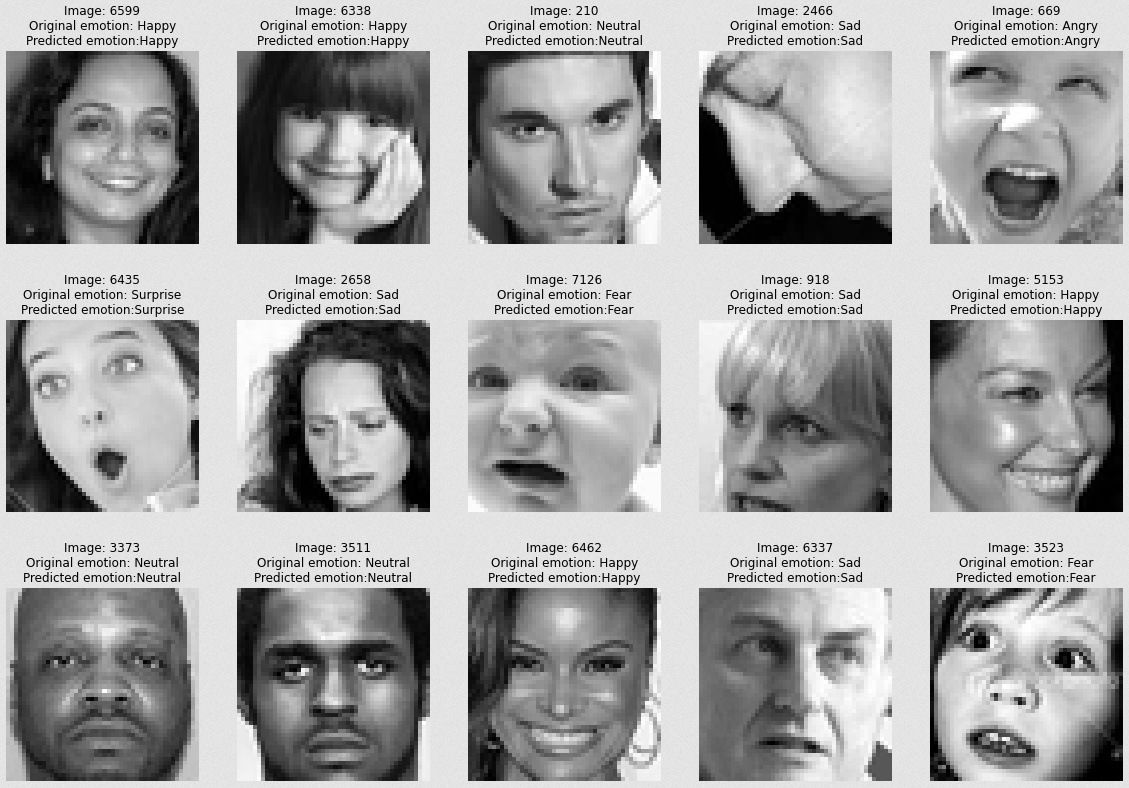
\includegraphics[scale=0.50]{images/modelOne/trueOne.png}
    \item Wronly predicted images\\
            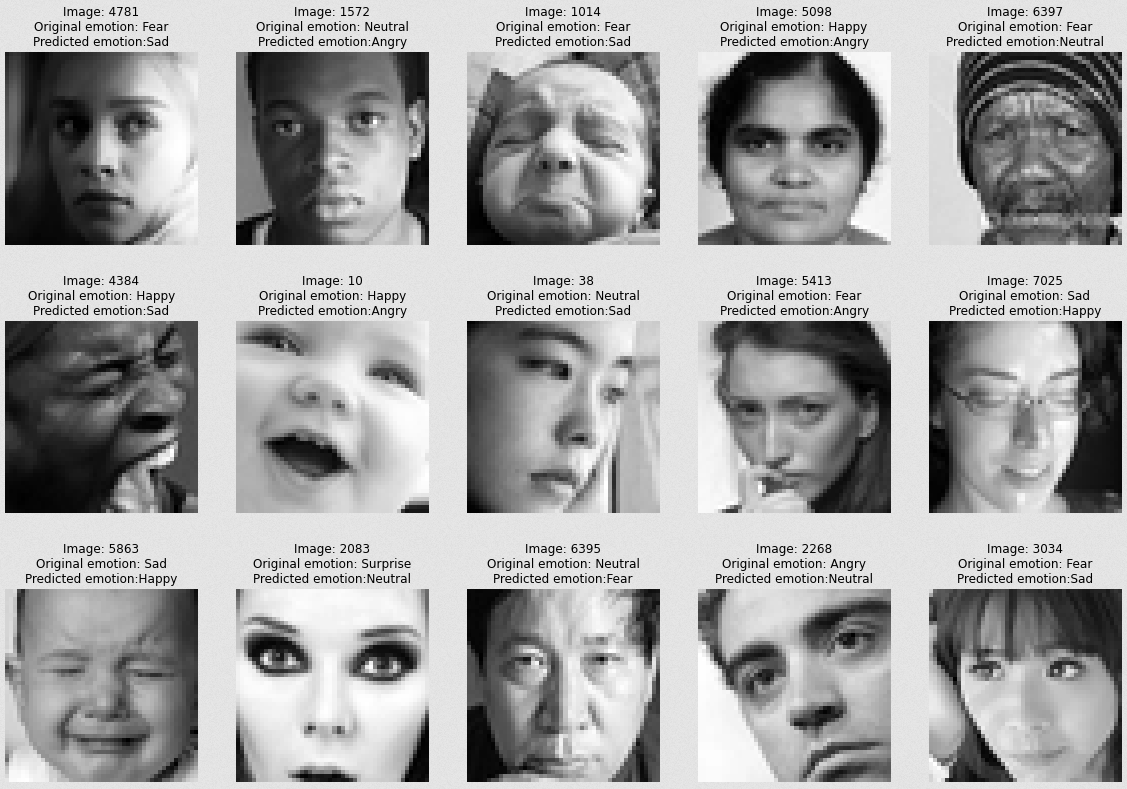
\includegraphics[scale=0.50]{images/modelOne/falseOne.png}
\end{itemize}
